% Options for packages loaded elsewhere
\PassOptionsToPackage{unicode}{hyperref}
\PassOptionsToPackage{hyphens}{url}
\PassOptionsToPackage{dvipsnames,svgnames,x11names}{xcolor}
%
\documentclass[
  11pt,
  a4paper,
  DIV=11,
  numbers=noendperiod]{scrartcl}

\usepackage{amsmath,amssymb}
\usepackage{iftex}
\ifPDFTeX
  \usepackage[T1]{fontenc}
  \usepackage[utf8]{inputenc}
  \usepackage{textcomp} % provide euro and other symbols
\else % if luatex or xetex
  \usepackage{unicode-math}
  \defaultfontfeatures{Scale=MatchLowercase}
  \defaultfontfeatures[\rmfamily]{Ligatures=TeX,Scale=1}
\fi
\usepackage{lmodern}
\ifPDFTeX\else  
    % xetex/luatex font selection
\fi
% Use upquote if available, for straight quotes in verbatim environments
\IfFileExists{upquote.sty}{\usepackage{upquote}}{}
\IfFileExists{microtype.sty}{% use microtype if available
  \usepackage[]{microtype}
  \UseMicrotypeSet[protrusion]{basicmath} % disable protrusion for tt fonts
}{}
\makeatletter
\@ifundefined{KOMAClassName}{% if non-KOMA class
  \IfFileExists{parskip.sty}{%
    \usepackage{parskip}
  }{% else
    \setlength{\parindent}{0pt}
    \setlength{\parskip}{6pt plus 2pt minus 1pt}}
}{% if KOMA class
  \KOMAoptions{parskip=half}}
\makeatother
\usepackage{xcolor}
\usepackage[lmargin=2cm,rmargin=2cm,tmargin=2cm,bmargin=2cm]{geometry}
\setlength{\emergencystretch}{3em} % prevent overfull lines
\setcounter{secnumdepth}{-\maxdimen} % remove section numbering
% Make \paragraph and \subparagraph free-standing
\makeatletter
\ifx\paragraph\undefined\else
  \let\oldparagraph\paragraph
  \renewcommand{\paragraph}{
    \@ifstar
      \xxxParagraphStar
      \xxxParagraphNoStar
  }
  \newcommand{\xxxParagraphStar}[1]{\oldparagraph*{#1}\mbox{}}
  \newcommand{\xxxParagraphNoStar}[1]{\oldparagraph{#1}\mbox{}}
\fi
\ifx\subparagraph\undefined\else
  \let\oldsubparagraph\subparagraph
  \renewcommand{\subparagraph}{
    \@ifstar
      \xxxSubParagraphStar
      \xxxSubParagraphNoStar
  }
  \newcommand{\xxxSubParagraphStar}[1]{\oldsubparagraph*{#1}\mbox{}}
  \newcommand{\xxxSubParagraphNoStar}[1]{\oldsubparagraph{#1}\mbox{}}
\fi
\makeatother

\usepackage{color}
\usepackage{fancyvrb}
\newcommand{\VerbBar}{|}
\newcommand{\VERB}{\Verb[commandchars=\\\{\}]}
\DefineVerbatimEnvironment{Highlighting}{Verbatim}{commandchars=\\\{\}}
% Add ',fontsize=\small' for more characters per line
\usepackage{framed}
\definecolor{shadecolor}{RGB}{241,243,245}
\newenvironment{Shaded}{\begin{snugshade}}{\end{snugshade}}
\newcommand{\AlertTok}[1]{\textcolor[rgb]{0.68,0.00,0.00}{#1}}
\newcommand{\AnnotationTok}[1]{\textcolor[rgb]{0.37,0.37,0.37}{#1}}
\newcommand{\AttributeTok}[1]{\textcolor[rgb]{0.40,0.45,0.13}{#1}}
\newcommand{\BaseNTok}[1]{\textcolor[rgb]{0.68,0.00,0.00}{#1}}
\newcommand{\BuiltInTok}[1]{\textcolor[rgb]{0.00,0.23,0.31}{#1}}
\newcommand{\CharTok}[1]{\textcolor[rgb]{0.13,0.47,0.30}{#1}}
\newcommand{\CommentTok}[1]{\textcolor[rgb]{0.37,0.37,0.37}{#1}}
\newcommand{\CommentVarTok}[1]{\textcolor[rgb]{0.37,0.37,0.37}{\textit{#1}}}
\newcommand{\ConstantTok}[1]{\textcolor[rgb]{0.56,0.35,0.01}{#1}}
\newcommand{\ControlFlowTok}[1]{\textcolor[rgb]{0.00,0.23,0.31}{\textbf{#1}}}
\newcommand{\DataTypeTok}[1]{\textcolor[rgb]{0.68,0.00,0.00}{#1}}
\newcommand{\DecValTok}[1]{\textcolor[rgb]{0.68,0.00,0.00}{#1}}
\newcommand{\DocumentationTok}[1]{\textcolor[rgb]{0.37,0.37,0.37}{\textit{#1}}}
\newcommand{\ErrorTok}[1]{\textcolor[rgb]{0.68,0.00,0.00}{#1}}
\newcommand{\ExtensionTok}[1]{\textcolor[rgb]{0.00,0.23,0.31}{#1}}
\newcommand{\FloatTok}[1]{\textcolor[rgb]{0.68,0.00,0.00}{#1}}
\newcommand{\FunctionTok}[1]{\textcolor[rgb]{0.28,0.35,0.67}{#1}}
\newcommand{\ImportTok}[1]{\textcolor[rgb]{0.00,0.46,0.62}{#1}}
\newcommand{\InformationTok}[1]{\textcolor[rgb]{0.37,0.37,0.37}{#1}}
\newcommand{\KeywordTok}[1]{\textcolor[rgb]{0.00,0.23,0.31}{\textbf{#1}}}
\newcommand{\NormalTok}[1]{\textcolor[rgb]{0.00,0.23,0.31}{#1}}
\newcommand{\OperatorTok}[1]{\textcolor[rgb]{0.37,0.37,0.37}{#1}}
\newcommand{\OtherTok}[1]{\textcolor[rgb]{0.00,0.23,0.31}{#1}}
\newcommand{\PreprocessorTok}[1]{\textcolor[rgb]{0.68,0.00,0.00}{#1}}
\newcommand{\RegionMarkerTok}[1]{\textcolor[rgb]{0.00,0.23,0.31}{#1}}
\newcommand{\SpecialCharTok}[1]{\textcolor[rgb]{0.37,0.37,0.37}{#1}}
\newcommand{\SpecialStringTok}[1]{\textcolor[rgb]{0.13,0.47,0.30}{#1}}
\newcommand{\StringTok}[1]{\textcolor[rgb]{0.13,0.47,0.30}{#1}}
\newcommand{\VariableTok}[1]{\textcolor[rgb]{0.07,0.07,0.07}{#1}}
\newcommand{\VerbatimStringTok}[1]{\textcolor[rgb]{0.13,0.47,0.30}{#1}}
\newcommand{\WarningTok}[1]{\textcolor[rgb]{0.37,0.37,0.37}{\textit{#1}}}

\providecommand{\tightlist}{%
  \setlength{\itemsep}{0pt}\setlength{\parskip}{0pt}}\usepackage{longtable,booktabs,array}
\usepackage{calc} % for calculating minipage widths
% Correct order of tables after \paragraph or \subparagraph
\usepackage{etoolbox}
\makeatletter
\patchcmd\longtable{\par}{\if@noskipsec\mbox{}\fi\par}{}{}
\makeatother
% Allow footnotes in longtable head/foot
\IfFileExists{footnotehyper.sty}{\usepackage{footnotehyper}}{\usepackage{footnote}}
\makesavenoteenv{longtable}
\usepackage{graphicx}
\makeatletter
\def\maxwidth{\ifdim\Gin@nat@width>\linewidth\linewidth\else\Gin@nat@width\fi}
\def\maxheight{\ifdim\Gin@nat@height>\textheight\textheight\else\Gin@nat@height\fi}
\makeatother
% Scale images if necessary, so that they will not overflow the page
% margins by default, and it is still possible to overwrite the defaults
% using explicit options in \includegraphics[width, height, ...]{}
\setkeys{Gin}{width=\maxwidth,height=\maxheight,keepaspectratio}
% Set default figure placement to htbp
\makeatletter
\def\fps@figure{htbp}
\makeatother

\KOMAoption{captions}{tableheading}
\makeatletter
\@ifpackageloaded{caption}{}{\usepackage{caption}}
\AtBeginDocument{%
\ifdefined\contentsname
  \renewcommand*\contentsname{Table of contents}
\else
  \newcommand\contentsname{Table of contents}
\fi
\ifdefined\listfigurename
  \renewcommand*\listfigurename{List of Figures}
\else
  \newcommand\listfigurename{List of Figures}
\fi
\ifdefined\listtablename
  \renewcommand*\listtablename{List of Tables}
\else
  \newcommand\listtablename{List of Tables}
\fi
\ifdefined\figurename
  \renewcommand*\figurename{Figure}
\else
  \newcommand\figurename{Figure}
\fi
\ifdefined\tablename
  \renewcommand*\tablename{Table}
\else
  \newcommand\tablename{Table}
\fi
}
\@ifpackageloaded{float}{}{\usepackage{float}}
\floatstyle{ruled}
\@ifundefined{c@chapter}{\newfloat{codelisting}{h}{lop}}{\newfloat{codelisting}{h}{lop}[chapter]}
\floatname{codelisting}{Listing}
\newcommand*\listoflistings{\listof{codelisting}{List of Listings}}
\makeatother
\makeatletter
\makeatother
\makeatletter
\@ifpackageloaded{caption}{}{\usepackage{caption}}
\@ifpackageloaded{subcaption}{}{\usepackage{subcaption}}
\makeatother

\ifLuaTeX
  \usepackage{selnolig}  % disable illegal ligatures
\fi
\usepackage{bookmark}

\IfFileExists{xurl.sty}{\usepackage{xurl}}{} % add URL line breaks if available
\urlstyle{same} % disable monospaced font for URLs
\hypersetup{
  colorlinks=true,
  linkcolor={blue},
  filecolor={Maroon},
  citecolor={Blue},
  urlcolor={Blue},
  pdfcreator={LaTeX via pandoc}}


\author{}
\date{}

\begin{document}


\begin{center}
\includegraphics{docs/kowalski-analysis-thinking.gif}
\end{center}

\section{Library Preparation}\label{library-preparation}

\begin{Shaded}
\begin{Highlighting}[]
\FunctionTok{library}\NormalTok{(dplyr)}
\FunctionTok{library}\NormalTok{(ggplot2)}
\FunctionTok{library}\NormalTok{(tidyr)}
\FunctionTok{library}\NormalTok{(scales)}
\FunctionTok{library}\NormalTok{(readr)}
\FunctionTok{library}\NormalTok{(readxl)}
\FunctionTok{library}\NormalTok{(ggthemes)}
\FunctionTok{library}\NormalTok{(forcats)}
\end{Highlighting}
\end{Shaded}

\section{ANALYSIS OF CO2 EMISSION FROM TRANSPORT DATA
(my\_data3)}\label{analysis-of-co2-emission-from-transport-data-my_data3}

my\_data3 will be used for this part of analysis. Therefore, here is the
general information that's needed:

\begin{Shaded}
\begin{Highlighting}[]
\FunctionTok{str}\NormalTok{(my\_data3)}
\end{Highlighting}
\end{Shaded}

\begin{verbatim}
'data.frame':   2232 obs. of  4 variables:
 $ entity                 : chr  "Afghanistan" "Africa" "Albania" "Algeria" ...
 $ code                   : chr  "AFG" "" "ALB" "DZA" ...
 $ year                   : int  2011 2011 2011 2011 2011 2011 2011 2011 2011 2011 ...
 $ transport_co2_emissions: num  6.71e+06 2.68e+08 2.36e+06 3.42e+07 6.28e+06 ...
\end{verbatim}

\textbf{entity:} A character column in my\_data3 data set which
represents the countries, continents, some income levels and the world.

\textbf{code:} A character column in my\_data3 data set which represents
the codes of the countries. (There are no codes for non-countries)

\textbf{year:} An integer column in my\_data3 data set which represents
the year.

\textbf{transport\_co2\_emissions:} A numeric column in my\_data3 data
set which represents the total carbon emission in tons.

\subsection{Country Based Mean Transportation CO2
Emission}\label{country-based-mean-transportation-co2-emission}

Let's take a look at the top 20 countries' mean transportation
carbondioxide emission from 2011 to 2021. To do this, the
\textbf{entity} column of my\_data3 has tidied to exclude the entities
that are non-countries.

\begin{Shaded}
\begin{Highlighting}[]
\NormalTok{non\_countries }\OtherTok{\textless{}{-}} \FunctionTok{c}\NormalTok{(}
  \StringTok{"World"}\NormalTok{, }
  \StringTok{"Upper{-}middle{-}income countries"}\NormalTok{, }
  \StringTok{"Lower{-}middle{-}income countries"}\NormalTok{, }
  \StringTok{"Low{-}income countries"}\NormalTok{, }
  \StringTok{"High{-}income countries"}\NormalTok{, }
  \StringTok{"European Union (27)"}\NormalTok{, }
  \StringTok{"Europe"}\NormalTok{, }
  \StringTok{"Asia"}\NormalTok{, }
  \StringTok{"Africa"}\NormalTok{,}
  \StringTok{"North America"}\NormalTok{,}
  \StringTok{"South America"}\NormalTok{,}
  \StringTok{"Oceania"}
\NormalTok{)}

\NormalTok{mean\_co2\_emission\_by\_country }\OtherTok{\textless{}{-}}\NormalTok{ my\_data3 }\SpecialCharTok{|\textgreater{}} 
  \FunctionTok{filter}\NormalTok{(}\SpecialCharTok{!}\NormalTok{entity }\SpecialCharTok{\%in\%}\NormalTok{ non\_countries) }\SpecialCharTok{|\textgreater{}}
  \FunctionTok{group\_by}\NormalTok{(entity) }\SpecialCharTok{|\textgreater{}}
  \FunctionTok{summarize}\NormalTok{(}\AttributeTok{mean\_co2\_emission\_per\_year =} \FunctionTok{mean}\NormalTok{(transport\_co2\_emissions,}
                                              \AttributeTok{na.rm =} \ConstantTok{TRUE}\NormalTok{)) }\SpecialCharTok{|\textgreater{}}
  \FunctionTok{mutate}\NormalTok{(}\AttributeTok{entity\_lumped =} \FunctionTok{fct\_lump\_n}\NormalTok{(entity, }\AttributeTok{n =} \DecValTok{20}\NormalTok{,}
                                    \AttributeTok{w =}\NormalTok{ mean\_co2\_emission\_per\_year)) }\SpecialCharTok{|\textgreater{}}
  \FunctionTok{group\_by}\NormalTok{(entity\_lumped) }\SpecialCharTok{|\textgreater{}}
  \FunctionTok{summarize}\NormalTok{(}\AttributeTok{mean\_co2\_emission\_per\_year =} \FunctionTok{mean}\NormalTok{(mean\_co2\_emission\_per\_year,}
                                              \AttributeTok{na.rm =} \ConstantTok{TRUE}\NormalTok{), }\AttributeTok{.groups =} \StringTok{"drop"}\NormalTok{)}

\FunctionTok{head}\NormalTok{(mean\_co2\_emission\_by\_country)}
\end{Highlighting}
\end{Shaded}

\begin{verbatim}
# A tibble: 6 x 2
  entity_lumped mean_co2_emission_per_year
  <fct>                              <dbl>
1 Australia                      92412727.
2 Brazil                        198190000 
3 Canada                        169276364.
4 China                         830712727.
5 France                        124309090 
6 Germany                       154080000 
\end{verbatim}

Note that to be able to see the mean carbondioxide emission of
\textbf{the rest of the world}, it is combined into the observation
\textbf{Other}.

It's needed to see the transportation carbondioxide emission levels of
countries through the years to get more information about them. Below,
the amounts of some of those 20 countries' (which are chosen
specifically by team NRG) mean transportation carbondioxide emission (in
tons) are displayed in the graph with the tidied version of my\_data3.

\begin{Shaded}
\begin{Highlighting}[]
\FunctionTok{ggplot}\NormalTok{(mean\_co2\_emission\_by\_country, }\FunctionTok{aes}\NormalTok{(}\AttributeTok{x =} \FunctionTok{reorder}\NormalTok{(entity\_lumped, mean\_co2\_emission\_per\_year),}\AttributeTok{y =}\NormalTok{ mean\_co2\_emission\_per\_year,}
                                         \AttributeTok{fill =}\NormalTok{ entity\_lumped)) }\SpecialCharTok{+}
\CommentTok{\# AI generated content based on the prompt: I want to plot a graph showing the}
\CommentTok{\# highest mean carbondioxide emission on the top, lowest on the bottom.}
\CommentTok{\# Can you aprovide a code? I think there is a reorder() function}
\CommentTok{\# that could help.}
  \FunctionTok{geom\_col}\NormalTok{(}\AttributeTok{width =} \FloatTok{0.5}\NormalTok{) }\SpecialCharTok{+}
  \FunctionTok{scale\_y\_continuous}\NormalTok{(}\AttributeTok{labels =} \FunctionTok{label\_number}\NormalTok{(}\AttributeTok{scale =} \DecValTok{1}\NormalTok{, }\AttributeTok{accuracy =} \DecValTok{1}\NormalTok{)) }\SpecialCharTok{+}
\CommentTok{\# AI generated content based on the prompt: Values are shown as a scientific}
\CommentTok{\# notation, I want to show them with a standard notation.}
  \FunctionTok{coord\_flip}\NormalTok{() }\SpecialCharTok{+}
  \FunctionTok{labs}\NormalTok{(}\AttributeTok{x =} \StringTok{"Country"}\NormalTok{,}
       \AttributeTok{y =} \StringTok{"Mean CO2 Emission"}\NormalTok{,}
       \AttributeTok{title =} \StringTok{"Mean CO2 Emission by Country"}\NormalTok{,}
       \AttributeTok{subtitle =} \StringTok{"From 2011 to 2021 (in tons)"}\NormalTok{) }\SpecialCharTok{+}
  \FunctionTok{theme\_light}\NormalTok{() }\SpecialCharTok{+}
  \FunctionTok{theme}\NormalTok{(}\AttributeTok{legend.position =} \StringTok{"none"}\NormalTok{)}
\end{Highlighting}
\end{Shaded}

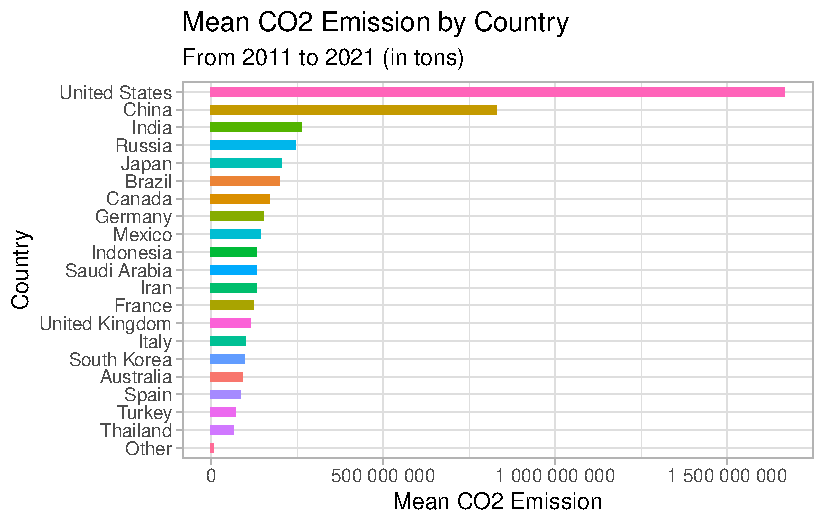
\includegraphics{analysis_files/figure-pdf/unnamed-chunk-4-1.pdf}

\textbf{Conclusions:}

\begin{itemize}
\item
  The histogram above clearly demonstrates that per capita CO₂ emissions
  in both the United States and China are significantly higher than the
  global average. This disparity has been one of the primary drivers
  behind the recent surge in renewable energy investments and efforts to
  move away from fossil fuels in both countries.
\item
  High emission levels have placed immense pressure on the United States
  and China to address climate change, accelerating their transition to
  sustainable energy sources.
\item
  The renewable energy initiatives undertaken by these two nations have
  created a significant domino effect worldwide, propelling the global
  shift toward the sustainability era. These efforts are not only aimed
  at reducing their own high emission levels but also serve as an
  example for other countries to transition to cleaner energy systems.
  One of the most tangible examples of this influence is the rapidly
  growing electric vehicle (EV) sector, driven by the United States as a
  hub of technological innovation and China as the world's largest
  manufacturer and market for EVs.
\item
  \textbf{The big majority} of mean transportation carbondioxide
  emissions consisted of top 20 countries.
\item
  \textbf{Turkey} is \textbf{19th country} with the largest mean
  transportation carbondioxide emission level.
\end{itemize}

After this plot, the group has chosen specific countries to explore
their behaviour over time. \textbf{United States and China} has chosen
for being in first two place in the mean carbondioxide emission
standings, \textbf{Norway and Denmark} for not being in top 20 countries
list, and even they have been successful at decreasing their emission,
\textbf{Turkey and Japan} to investigate the important parameters that
carbondioxide emission is dependent.

\begin{Shaded}
\begin{Highlighting}[]
\NormalTok{top6\_countries }\OtherTok{\textless{}{-}} \FunctionTok{c}\NormalTok{(}\StringTok{"United States"}\NormalTok{, }\StringTok{"Norway"}\NormalTok{, }\StringTok{"Denmark"}\NormalTok{, }\StringTok{"China"}\NormalTok{, }\StringTok{"Japan"}\NormalTok{,}
                    \StringTok{"Turkey"}\NormalTok{)}

\NormalTok{emission\_by\_country }\OtherTok{\textless{}{-}}\NormalTok{ my\_data3 }\SpecialCharTok{|\textgreater{}}
  \FunctionTok{filter}\NormalTok{(entity }\SpecialCharTok{\%in\%}\NormalTok{ top6\_countries)}

\FunctionTok{head}\NormalTok{(emission\_by\_country)}
\end{Highlighting}
\end{Shaded}

\begin{verbatim}
         entity code year transport_co2_emissions
1         China  CHN 2011               621890000
2       Denmark  DNK 2011                12640000
3         Japan  JPN 2011               223030000
4        Norway  NOR 2011                14980000
5        Turkey  TUR 2011                44000000
6 United States  USA 2011              1633590000
\end{verbatim}

Here, \textbf{emission\_by\_country} is the more tidied version of
my\_data3 in which the interested countries' carbondioxide emission is
analyzed.

The line plot below visualizes how much tons of carbondioxide did each
selected country emit:

\begin{Shaded}
\begin{Highlighting}[]
\FunctionTok{ggplot}\NormalTok{(emission\_by\_country, }\FunctionTok{aes}\NormalTok{(}\AttributeTok{x =}\NormalTok{ year, }\AttributeTok{y =}\NormalTok{ transport\_co2\_emissions, }\AttributeTok{color =}\NormalTok{ entity)) }\SpecialCharTok{+}
  \FunctionTok{geom\_line}\NormalTok{(}\AttributeTok{size =} \DecValTok{1}\NormalTok{) }\SpecialCharTok{+}
  \FunctionTok{scale\_y\_continuous}\NormalTok{(}
    \AttributeTok{trans =} \StringTok{"log10"}\NormalTok{,}
    \AttributeTok{breaks =} \FunctionTok{c}\NormalTok{(}\DecValTok{1}\NormalTok{, }\DecValTok{10}\NormalTok{, }\DecValTok{100}\NormalTok{, }\DecValTok{1000}\NormalTok{, }\DecValTok{10000}\NormalTok{, }\DecValTok{100000}\NormalTok{, }\DecValTok{1000000}\NormalTok{, }\DecValTok{10000000}\NormalTok{, }\DecValTok{100000000}\NormalTok{, }\DecValTok{1000000000}\NormalTok{, }\DecValTok{10000000000}\NormalTok{),}
    \AttributeTok{labels =} \FunctionTok{c}\NormalTok{(}\StringTok{"1"}\NormalTok{, }\StringTok{"10"}\NormalTok{, }\StringTok{"100"}\NormalTok{, }\StringTok{"1K"}\NormalTok{, }\StringTok{"10K"}\NormalTok{, }\StringTok{"100K"}\NormalTok{, }\StringTok{"1M"}\NormalTok{, }\StringTok{"10M"}\NormalTok{, }\StringTok{"100M"}\NormalTok{, }\StringTok{"1B"}\NormalTok{, }\StringTok{"10B"}\NormalTok{)}
\NormalTok{  ) }\SpecialCharTok{+}
  \FunctionTok{scale\_x\_continuous}\NormalTok{(}\AttributeTok{breaks =} \DecValTok{2011}\SpecialCharTok{:}\DecValTok{2021}\NormalTok{) }\SpecialCharTok{+}
  \FunctionTok{facet\_wrap}\NormalTok{(}\SpecialCharTok{\textasciitilde{}}\NormalTok{ entity) }\SpecialCharTok{+}
  \FunctionTok{labs}\NormalTok{(}\AttributeTok{x =} \StringTok{"Year"}\NormalTok{, }
       \AttributeTok{y =} \StringTok{"CO2 Emission"}\NormalTok{,}
       \AttributeTok{title =} \StringTok{"Carbondioxide Emissions by Entity (Logarithmic Scale)"}\NormalTok{,}
       \AttributeTok{subtitle =} \StringTok{"From 2011 to 2021 (in tons)"}
\NormalTok{       ) }\SpecialCharTok{+}
  \FunctionTok{theme\_bw}\NormalTok{() }\SpecialCharTok{+}
  \FunctionTok{theme}\NormalTok{(}\AttributeTok{legend.position =} \StringTok{"none"}\NormalTok{,}
        \AttributeTok{axis.text.x =} \FunctionTok{element\_text}\NormalTok{(}\AttributeTok{angle =} \DecValTok{90}\NormalTok{, }\AttributeTok{hjust =} \DecValTok{1}\NormalTok{))}
\end{Highlighting}
\end{Shaded}

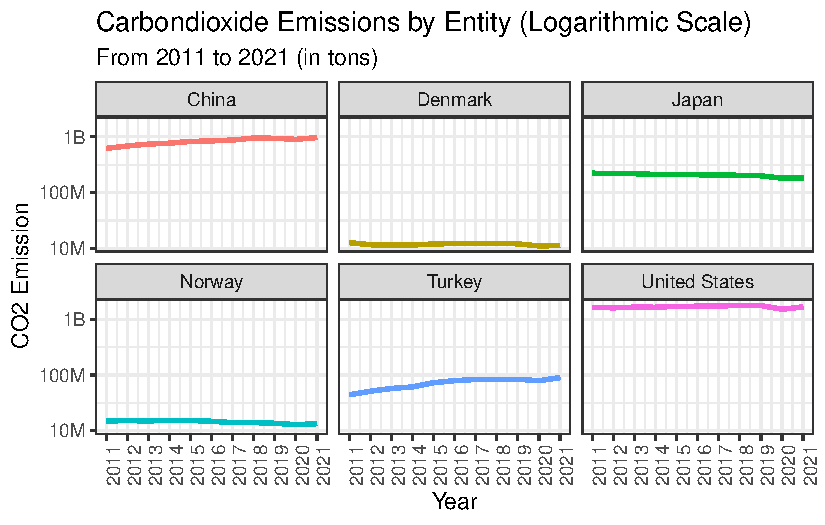
\includegraphics{analysis_files/figure-pdf/unnamed-chunk-6-1.pdf}

Here are some observations from this graph:

\begin{enumerate}
\def\labelenumi{\arabic{enumi}.}
\item
  It can be observed that there is a persistent increase in the
  carbondioxide emission levels in \textbf{Turkey and China}. China is
  very close to emit one billion tons of carbondioxide.
\item
  \textbf{Denmark} has decreased its carbondioxide emission level after
  a 10-year horizon. \textbf{Japan and Norway} has a considerable
  decreasing trend in its carbondioxide emission level.
\item
  \textbf{USA} has the highest carbondioxide emission compared to
  others, exceeding one billion tons of carbondioxide.
\end{enumerate}

This graph compares those 6 countries very well, but it's not possible
to see the trends for each of them. Therefore, the line plot below has
been made to display the \textbf{trend} in the transportation
carbondioxide emission levels of those exactly same countries to make a
comparison.

\begin{Shaded}
\begin{Highlighting}[]
\FunctionTok{ggplot}\NormalTok{(emission\_by\_country, }\FunctionTok{aes}\NormalTok{(}\AttributeTok{x =}\NormalTok{ year, }\AttributeTok{y =}\NormalTok{ transport\_co2\_emissions, }\AttributeTok{color =}\NormalTok{ entity)) }\SpecialCharTok{+}
  \FunctionTok{geom\_line}\NormalTok{(}\AttributeTok{size =} \DecValTok{1}\NormalTok{) }\SpecialCharTok{+}
  \FunctionTok{scale\_y\_continuous}\NormalTok{(}
    \AttributeTok{trans =} \StringTok{"log10"}\NormalTok{,}
    \AttributeTok{breaks =} \FunctionTok{c}\NormalTok{(}\DecValTok{1}\NormalTok{, }\DecValTok{10}\NormalTok{, }\DecValTok{100}\NormalTok{, }\DecValTok{1000}\NormalTok{, }\DecValTok{10000}\NormalTok{, }\DecValTok{100000}\NormalTok{, }\DecValTok{1000000}\NormalTok{, }\DecValTok{10000000}\NormalTok{, }\DecValTok{100000000}\NormalTok{, }\DecValTok{1000000000}\NormalTok{, }\DecValTok{10000000000}\NormalTok{),}
    \AttributeTok{labels =} \FunctionTok{c}\NormalTok{(}\StringTok{"1"}\NormalTok{, }\StringTok{"10"}\NormalTok{, }\StringTok{"100"}\NormalTok{, }\StringTok{"1K"}\NormalTok{, }\StringTok{"10K"}\NormalTok{, }\StringTok{"100K"}\NormalTok{, }\StringTok{"1M"}\NormalTok{, }\StringTok{"10M"}\NormalTok{, }\StringTok{"100M"}\NormalTok{, }\StringTok{"1B"}\NormalTok{, }\StringTok{"10B"}\NormalTok{)}
\NormalTok{  ) }\SpecialCharTok{+}
  \FunctionTok{scale\_x\_continuous}\NormalTok{(}\AttributeTok{breaks =} \DecValTok{2011}\SpecialCharTok{:}\DecValTok{2021}\NormalTok{) }\SpecialCharTok{+}
  \FunctionTok{facet\_wrap}\NormalTok{(}\SpecialCharTok{\textasciitilde{}}\NormalTok{ entity, }\AttributeTok{scale =} \StringTok{"free\_y"}\NormalTok{) }\SpecialCharTok{+}
  \FunctionTok{labs}\NormalTok{(}\AttributeTok{x =} \StringTok{"Year"}\NormalTok{, }
       \AttributeTok{y =} \StringTok{"CO2 Emission"}\NormalTok{,}
       \AttributeTok{title =} \StringTok{"Carbondioxide Emissions by Entity (Logarithmic Scale)"}\NormalTok{,}
       \AttributeTok{subtitle =} \StringTok{"Carbondioxide emission trends from 2011 to 2021"}
\NormalTok{       ) }\SpecialCharTok{+}
  \FunctionTok{theme\_bw}\NormalTok{() }\SpecialCharTok{+}
  \FunctionTok{theme}\NormalTok{(}\AttributeTok{legend.position =} \StringTok{"none"}\NormalTok{,}
        \AttributeTok{axis.text.x =} \FunctionTok{element\_text}\NormalTok{(}\AttributeTok{angle =} \DecValTok{90}\NormalTok{, }\AttributeTok{hjust =} \DecValTok{1}\NormalTok{))}
\end{Highlighting}
\end{Shaded}

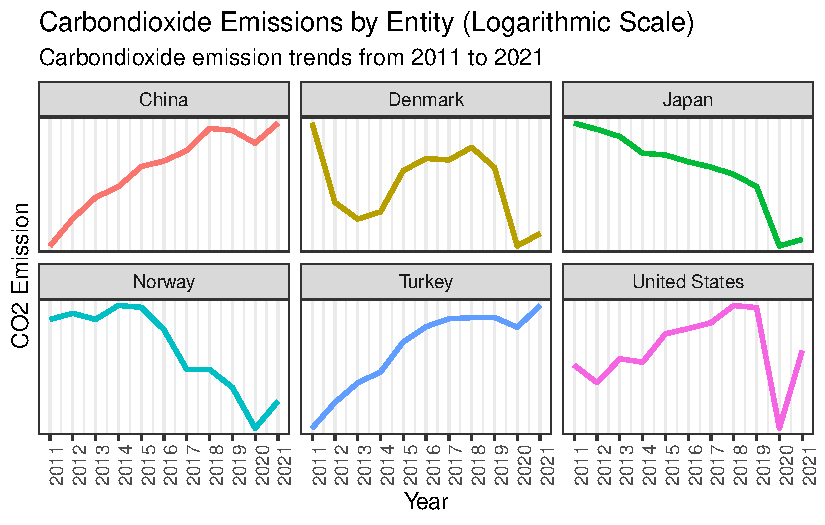
\includegraphics{analysis_files/figure-pdf/unnamed-chunk-7-1.pdf}

Here are some observations from this graph:

\begin{enumerate}
\def\labelenumi{\arabic{enumi}.}
\item
  It can be observed that China's, USA's and Turkey's total
  transportation carbondioxide emission level have an increasing trend
  over years while Denmark's, Norway's and Japan's have a decreasing
  trend.
\item
  All of the countries have a clear reduction of total transportation
  carbondioxide emission level \textbf{in 2020}. This is the effect of
  \textbf{COVID-19 pandemic} which causes a \textbf{V-shaped pattern}
  for all countries listed.
\end{enumerate}

This graphs gives a lot of information about transportation
carbondioxide emission levels of those countries. But is it correct to
make a decision just by looking at these graphs only? May population be
the reason of some countries' low/high total transportation
carbondioxide emission levels? Let's analyze it.

\section{ANALYSIS OF THE POPULATION DATA ALONG WITH CO2 EMISSIONS
(my\_data3 \&
my\_data8)}\label{analysis-of-the-population-data-along-with-co2-emissions-my_data3-my_data8}

\subsection{The Effect of Population on Transport CO2
Emissions}\label{the-effect-of-population-on-transport-co2-emissions}

\begin{Shaded}
\begin{Highlighting}[]
\FunctionTok{str}\NormalTok{(my\_data8)}
\end{Highlighting}
\end{Shaded}

\begin{verbatim}
'data.frame':   2816 obs. of  3 variables:
 $ entity    : chr  "Afghanistan" "Afghanistan" "Afghanistan" "Afghanistan" ...
 $ year      : int  2011 2012 2013 2014 2015 2016 2017 2018 2019 2020 ...
 $ population: num  29347709 30560036 31622708 32792527 33831765 ...
\end{verbatim}

\textbf{entity:} A character column in my\_data3 data set which
represents the countries.

\textbf{year:} An integer column in my\_data3 data set which represents
the year.

\textbf{population:} A numeric column in my\_data8 data set which
represents the population of each country.

\begin{Shaded}
\begin{Highlighting}[]
\NormalTok{countries\_selected }\OtherTok{\textless{}{-}} \FunctionTok{c}\NormalTok{(}\StringTok{"United States"}\NormalTok{, }\StringTok{"Norway"}\NormalTok{, }\StringTok{"Denmark"}\NormalTok{, }\StringTok{"China"}\NormalTok{, }\StringTok{"Japan"}\NormalTok{, }\StringTok{"Turkey"}\NormalTok{)}

\NormalTok{pop\_n\_co2 }\OtherTok{\textless{}{-}}\NormalTok{ my\_data3 }\SpecialCharTok{|\textgreater{}}
  \FunctionTok{full\_join}\NormalTok{(my\_data8, }\AttributeTok{by =} \FunctionTok{c}\NormalTok{(}\StringTok{"entity"} \OtherTok{=} \StringTok{"entity"}\NormalTok{, }\StringTok{"year"} \OtherTok{=} \StringTok{"year"}\NormalTok{)) }\SpecialCharTok{|\textgreater{}}
  \FunctionTok{replace\_na}\NormalTok{(}\FunctionTok{list}\NormalTok{(}\AttributeTok{transport\_co2\_emissions =} \DecValTok{0}\NormalTok{, }\AttributeTok{population =} \DecValTok{0}\NormalTok{))}
\FunctionTok{head}\NormalTok{(pop\_n\_co2)}
\end{Highlighting}
\end{Shaded}

\begin{verbatim}
               entity code year transport_co2_emissions population
1         Afghanistan  AFG 2011                 6710000   29347709
2              Africa      2011               267989980          0
3             Albania  ALB 2011                 2360000    2911500
4             Algeria  DZA 2011                34220000   36903375
5              Angola  AGO 2011                 6280000   24218358
6 Antigua and Barbuda  ATG 2011                  190000      86349
\end{verbatim}

Here, two data frames has been joined to include carbondioxide emissions
and population columns in one data frame and replace the NA values to
zero.

\begin{Shaded}
\begin{Highlighting}[]
\NormalTok{pop\_n\_co2 }\OtherTok{\textless{}{-}}\NormalTok{ pop\_n\_co2 }\SpecialCharTok{|\textgreater{}}
  \FunctionTok{mutate}\NormalTok{(}\AttributeTok{prop =}\NormalTok{ transport\_co2\_emissions }\SpecialCharTok{/}\NormalTok{ population) }\SpecialCharTok{|\textgreater{}}
  \FunctionTok{filter}\NormalTok{(entity }\SpecialCharTok{\%in\%}\NormalTok{ countries\_selected)}
\FunctionTok{head}\NormalTok{(pop\_n\_co2)}
\end{Highlighting}
\end{Shaded}

\begin{verbatim}
         entity code year transport_co2_emissions population      prop
1         China  CHN 2011               621890000 1360250657 0.4571878
2       Denmark  DNK 2011                12640000    5570846 2.2689552
3         Japan  JPN 2011               223030000  128096431 1.7411102
4        Norway  NOR 2011                14980000    4952968 3.0244492
5        Turkey  TUR 2011                44000000   74215200 0.5928705
6 United States  USA 2011              1633590000  314105078 5.2007755
\end{verbatim}

After that, the data has filtered by selected countries.

The line plot below visualizes the selected countries' carbondioxide
emission per person on the average over time:

\begin{Shaded}
\begin{Highlighting}[]
\FunctionTok{ggplot}\NormalTok{(pop\_n\_co2, }\FunctionTok{aes}\NormalTok{(}\AttributeTok{x =}\NormalTok{ year, }\AttributeTok{y =}\NormalTok{ prop, }\AttributeTok{color =}\NormalTok{ entity)) }\SpecialCharTok{+}
  \FunctionTok{geom\_line}\NormalTok{(}\AttributeTok{size =} \DecValTok{1}\NormalTok{) }\SpecialCharTok{+}
  \FunctionTok{scale\_x\_continuous}\NormalTok{(}\AttributeTok{breaks =} \DecValTok{2011}\SpecialCharTok{:}\DecValTok{2021}\NormalTok{) }\SpecialCharTok{+}
  \FunctionTok{labs}\NormalTok{(}\AttributeTok{x =} \StringTok{"Year"}\NormalTok{,}
       \AttributeTok{y =} \StringTok{"CO2 Emission (in tons) / Population"}\NormalTok{,}
       \AttributeTok{title =} \StringTok{"CO2 Emission per Person"}\NormalTok{,}
       \AttributeTok{subtitle =} \StringTok{"Describes how much carbondioxide emission does a person}
\StringTok{       emits on the average (in tons)"}\NormalTok{,}
       \AttributeTok{color =} \StringTok{"Entity"}\NormalTok{)}
\end{Highlighting}
\end{Shaded}

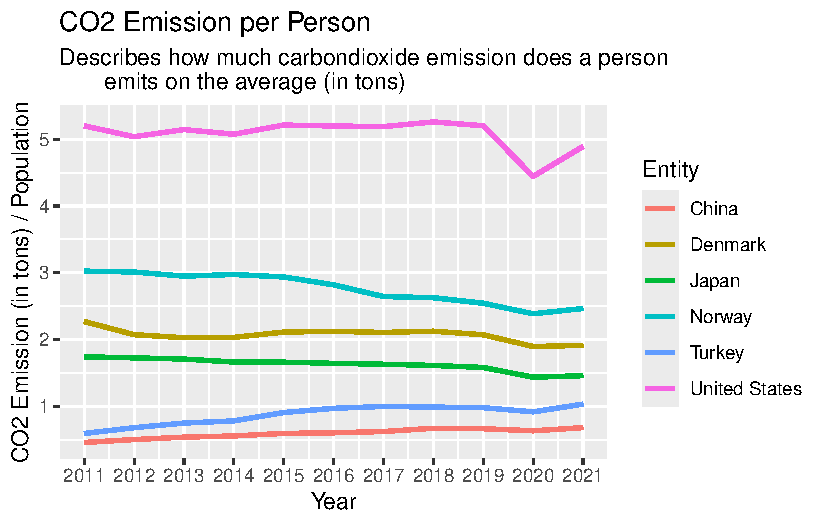
\includegraphics{analysis_files/figure-pdf/unnamed-chunk-11-1.pdf}

Here are some observations from this graph:

\begin{enumerate}
\def\labelenumi{\arabic{enumi}.}
\item
  When we analyze the transportation carbon emission per person, even
  China has the one of the highest total transportation carbondioxide
  emission, it can be seen that \textbf{China} has the lowest
  transportation carbondioxide emission per person among all other
  countries. While \textbf{USA} on the other hand, still has the highest
  level.
\item
  \textbf{Denmark's, Norway's and Japan's} transportation carbon
  emission per person have a \textbf{decreasing} trend.
\item
  \textbf{Turkey's} transportation carbon emission per person is
  \textbf{not high} but it has an \textbf{increasing} trend.
\item
  The decrease \textbf{in 2020} can be seen again.
\end{enumerate}

\section{GLOBAL EV SALES (my\_data2)}\label{global-ev-sales-my_data2}

\begin{Shaded}
\begin{Highlighting}[]
\FunctionTok{str}\NormalTok{(my\_data2)}
\end{Highlighting}
\end{Shaded}

\begin{verbatim}
spc_tbl_ [8,019 x 8] (S3: spec_tbl_df/tbl_df/tbl/data.frame)
 $ region    : chr [1:8019] "Australia" "Australia" "Australia" "Australia" ...
 $ category  : chr [1:8019] "Historical" "Historical" "Historical" "Historical" ...
 $ parameter : chr [1:8019] "EV stock share" "EV sales share" "EV sales" "EV stock" ...
 $ mode      : chr [1:8019] "Cars" "Cars" "Cars" "Cars" ...
 $ powertrain: chr [1:8019] "EV" "EV" "BEV" "BEV" ...
 $ year      : num [1:8019] 2011 2011 2011 2011 2011 ...
 $ unit      : chr [1:8019] "percent" "percent" "Vehicles" "Vehicles" ...
 $ value     : num [1:8019] 3.9e-04 6.5e-03 4.9e+01 4.9e+01 2.2e-02 ...
 - attr(*, "spec")=
  .. cols(
  ..   region = col_character(),
  ..   category = col_character(),
  ..   parameter = col_character(),
  ..   mode = col_character(),
  ..   powertrain = col_character(),
  ..   year = col_double(),
  ..   unit = col_character(),
  ..   value = col_double()
  .. )
 - attr(*, "problems")=<externalptr> 
\end{verbatim}

\textbf{region:} A character column in my\_data2 data set which
represents the countries and the world.

\textbf{category:} A character column in my\_data2 data set which
represents how the data has collected.

\textbf{parameter:} A character column in my\_data2 data set which
represents the parameter of the data collected.

\textbf{mode:} A character column in my\_data2 data set which represents
the vehicle types.

\textbf{powertrain:} A character column in my\_data2 data set which
represents how the vehicle gets its power from, a.k.a. type of the
powertrain that the vehicle uses which are EV, BEV, PHEV etc.

\textbf{year:} A numeric column in my\_data2 data set which represents
the year.

\textbf{unit:} A character column in my\_data2 data set which represents
the unit that is used.

\textbf{value:} A numeric column in my\_data2 data set which represents
the amount of the vehicles in unit.

\subsection{Sales of No Carbon
Vehicles}\label{sales-of-no-carbon-vehicles}

What about the countries' adoption on EV's? To be able to understand the
relationship between EV sales and transportation, my\_data2 is used. The
same countries are filtered from it.

The types of EV's are summarized below.

\begin{itemize}
\tightlist
\item
  Battery Electric Vehicle (BEV)
\item
  Plug-in Hybrid Electric Vehicle (PHEV)
\item
  Fuel Cell Electric Vehicle (FCEV)
\item
  Hybrid Electric Vehicle (HEV)
\item
  Mild Hybrid Vehicle (MHEV)
\end{itemize}

\textbf{BEV and FCEV} sales are analysed since they're the no carbon
ones.

\begin{Shaded}
\begin{Highlighting}[]
\NormalTok{my\_data2}\SpecialCharTok{$}\NormalTok{region[my\_data2}\SpecialCharTok{$}\NormalTok{region }\SpecialCharTok{==} \StringTok{"Turkiye"}\NormalTok{] }\OtherTok{\textless{}{-}} \StringTok{"Turkey"}
\CommentTok{\# AI generated content based on the prompt: In my R data frame, I have a region}
\CommentTok{\# column and I have seen that Turkey in one data set is written as Turkiye in}
\CommentTok{\# another data set so that I want to make Turkiye as Turkey. How can I change}
\CommentTok{\# it?}
\NormalTok{top6\_countries }\OtherTok{=} \FunctionTok{c}\NormalTok{(}\StringTok{"USA"}\NormalTok{, }\StringTok{"Norway"}\NormalTok{, }\StringTok{"Denmark"}\NormalTok{, }\StringTok{"China"}\NormalTok{, }\StringTok{"Japan"}\NormalTok{, }\StringTok{"Turkey"}\NormalTok{)}
\NormalTok{no\_carbon }\OtherTok{=} \FunctionTok{c}\NormalTok{(}\StringTok{"BEV"}\NormalTok{, }\StringTok{"FCEV"}\NormalTok{)}

\NormalTok{top6\_ev\_sales }\OtherTok{\textless{}{-}}\NormalTok{ my\_data2 }\SpecialCharTok{|\textgreater{}}
  \FunctionTok{filter}\NormalTok{(region }\SpecialCharTok{\%in\%}\NormalTok{ top6\_countries, parameter }\SpecialCharTok{==} \StringTok{"EV sales"}\NormalTok{, powertrain }\SpecialCharTok{\%in\%}\NormalTok{ no\_carbon)}

\NormalTok{top6\_ev\_sales }\SpecialCharTok{|\textgreater{}} \FunctionTok{mutate}\NormalTok{(}\AttributeTok{value =} \FunctionTok{as.numeric}\NormalTok{(}\FunctionTok{format}\NormalTok{(value, }\AttributeTok{scientific =} \ConstantTok{FALSE}\NormalTok{)))}
\end{Highlighting}
\end{Shaded}

\begin{verbatim}
# A tibble: 276 x 8
   region  category   parameter mode  powertrain  year unit     value
   <chr>   <chr>      <chr>     <chr> <chr>      <dbl> <chr>    <dbl>
 1 China   Historical EV sales  Buses BEV         2011 Vehicles   440
 2 China   Historical EV sales  Vans  BEV         2011 Vehicles   150
 3 China   Historical EV sales  Cars  BEV         2011 Vehicles  4800
 4 Denmark Historical EV sales  Vans  BEV         2011 Vehicles    23
 5 Denmark Historical EV sales  Cars  BEV         2011 Vehicles   420
 6 Denmark Historical EV sales  Buses BEV         2011 Vehicles     1
 7 Japan   Historical EV sales  Cars  BEV         2011 Vehicles 13000
 8 Japan   Historical EV sales  Buses BEV         2011 Vehicles     2
 9 Japan   Historical EV sales  Vans  BEV         2011 Vehicles   850
10 Norway  Historical EV sales  Vans  BEV         2011 Vehicles    42
# i 266 more rows
\end{verbatim}

\begin{Shaded}
\begin{Highlighting}[]
\FunctionTok{head}\NormalTok{(top6\_ev\_sales)}
\end{Highlighting}
\end{Shaded}

\begin{verbatim}
# A tibble: 6 x 8
  region  category   parameter mode  powertrain  year unit     value
  <chr>   <chr>      <chr>     <chr> <chr>      <dbl> <chr>    <dbl>
1 China   Historical EV sales  Buses BEV         2011 Vehicles   440
2 China   Historical EV sales  Vans  BEV         2011 Vehicles   150
3 China   Historical EV sales  Cars  BEV         2011 Vehicles  4800
4 Denmark Historical EV sales  Vans  BEV         2011 Vehicles    23
5 Denmark Historical EV sales  Cars  BEV         2011 Vehicles   420
6 Denmark Historical EV sales  Buses BEV         2011 Vehicles     1
\end{verbatim}

The line plot below visualizes how the EV Sales of Non-Carbon Vehicles
has evolved over the 10-year horizon:

\begin{Shaded}
\begin{Highlighting}[]
\NormalTok{top6\_ev\_sales }\SpecialCharTok{|\textgreater{}} \FunctionTok{group\_by}\NormalTok{(year, region, powertrain) }\SpecialCharTok{|\textgreater{}}
  \FunctionTok{summarize}\NormalTok{(}\AttributeTok{total\_sales =} \FunctionTok{sum}\NormalTok{(value, }\AttributeTok{na.rm =} \ConstantTok{TRUE}\NormalTok{), }\AttributeTok{.groups =} \StringTok{"drop"}\NormalTok{) }\SpecialCharTok{|\textgreater{}}
  \FunctionTok{ggplot}\NormalTok{(}\FunctionTok{aes}\NormalTok{(}\AttributeTok{x =}\NormalTok{ year, }\AttributeTok{y =}\NormalTok{ total\_sales, }\AttributeTok{color =}\NormalTok{ region, }\AttributeTok{linetype =}\NormalTok{ powertrain)) }\SpecialCharTok{+}
  \FunctionTok{geom\_line}\NormalTok{(}\AttributeTok{size =} \DecValTok{1}\NormalTok{) }\SpecialCharTok{+}
  \FunctionTok{scale\_x\_continuous}\NormalTok{(}\AttributeTok{breaks =} \DecValTok{2011}\SpecialCharTok{:}\DecValTok{2021}\NormalTok{) }\SpecialCharTok{+}
  \FunctionTok{scale\_y\_continuous}\NormalTok{(}\AttributeTok{trans =} \StringTok{"log10"}\NormalTok{,}
                     \AttributeTok{labels =} \FunctionTok{label\_number}\NormalTok{(}\AttributeTok{scale =} \DecValTok{1}\NormalTok{, }\AttributeTok{accuracy =} \DecValTok{1}\NormalTok{)}
\NormalTok{                     ) }\SpecialCharTok{+}
  \FunctionTok{labs}\NormalTok{(}\AttributeTok{x =} \StringTok{"Year"}\NormalTok{,}
       \AttributeTok{y =} \StringTok{"Sales"}\NormalTok{,}
       \AttributeTok{title =} \StringTok{"Sales of No Carbon Vehicles (Logarithmic Scale)"}\NormalTok{,}
       \AttributeTok{subtitle =} \StringTok{"The behaviour of the number of sales of vehicles that emit no carbon over time"}\NormalTok{,}
       \AttributeTok{color =} \StringTok{"Region"}\NormalTok{,}
       \AttributeTok{linetype =} \StringTok{"Powertrain Type"}
\NormalTok{  ) }\SpecialCharTok{+}
  \FunctionTok{facet\_wrap}\NormalTok{(}\SpecialCharTok{\textasciitilde{}}\NormalTok{ region) }\SpecialCharTok{+}
  \FunctionTok{theme\_light}\NormalTok{() }\SpecialCharTok{+}
  \FunctionTok{theme}\NormalTok{(}\AttributeTok{axis.text.x =} \FunctionTok{element\_text}\NormalTok{(}\AttributeTok{angle =} \DecValTok{90}\NormalTok{, }\AttributeTok{hjust =} \DecValTok{1}\NormalTok{)) }\SpecialCharTok{+}
  \FunctionTok{guides}\NormalTok{(}\AttributeTok{color =} \StringTok{"none"}\NormalTok{) }\CommentTok{\# AI generated content based on the prompt: I have two legends in the plot, I want to remove the region legend.}
\end{Highlighting}
\end{Shaded}

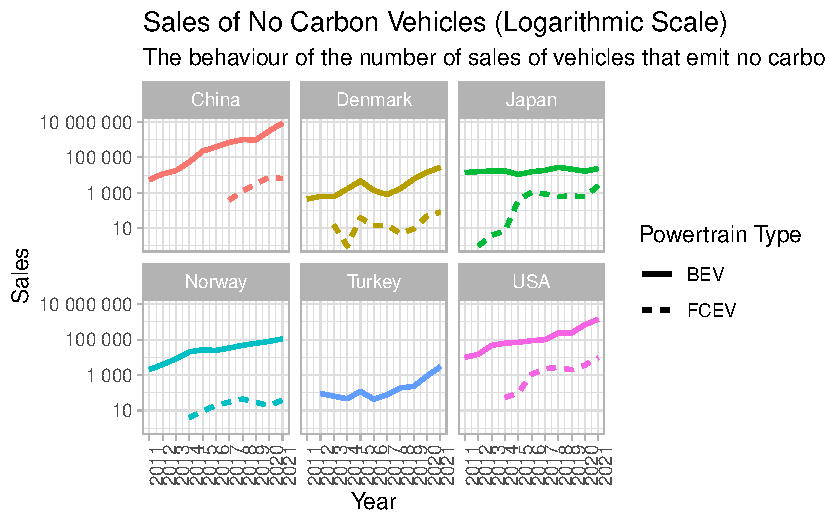
\includegraphics{analysis_files/figure-pdf/unnamed-chunk-14-1.pdf}

Here are some observations from this graph:

\begin{enumerate}
\def\labelenumi{\arabic{enumi}.}
\item
  All countries in the plot increased their non-carbon emitting vehicle
  sales after 10-year horizon. However, \textbf{Turkey} has not been
  adopted \textbf{FCEV's through 2021} yet, while the other countries
  are using \textbf{FCEV's} more year by year. \textbf{China} has
  started using \textbf{FCEV's} (in 2016) \textbf{later} than the others
  (in 2011-2014). It can be also observed that \textbf{BEV} sales has
  started \textbf{2012 in Turkey}.
\item
  \textbf{China} has increased its \textbf{BEV} and \textbf{FCEV} sales
  more than any other country, however from the last analyses we know
  that it couldn't make any big difference in total transportation
  carbondioxide emission since it's population is too high. On the other
  hand, \textbf{in Norway and Denmark}, \textbf{BEV's} and
  \textbf{FCEV's} has a \textbf{positive} effect on total transportation
  carbondioxide emission since their populations are much lower than
  \textbf{China}.
\item
  It can be seen that \textbf{Japan} didn't increase the sales of
  \textbf{BEV's}. Yet, they managed to decrease the total transportation
  carbondioxide emission by increasing the \textbf{FCEV} sales
  considerably, which means they have done some other applications.
\end{enumerate}

\subsection{The Relationship Between CO2 Emission \& Total EV Sales
(my\_data2 \&
my\_data3)}\label{the-relationship-between-co2-emission-total-ev-sales-my_data2-my_data3}

So, how carbondioxide emission has been affected by total EV sales?

For this part of analysis, \textbf{my\_data2} and \textbf{my\_data3}
will be used. The selected countries will be analyzed again.

\begin{Shaded}
\begin{Highlighting}[]
\NormalTok{countries\_selected }\OtherTok{\textless{}{-}} \FunctionTok{c}\NormalTok{(}\StringTok{"United States"}\NormalTok{, }\StringTok{"Norway"}\NormalTok{, }\StringTok{"Denmark"}\NormalTok{, }\StringTok{"China"}\NormalTok{, }\StringTok{"Japan"}\NormalTok{, }\StringTok{"Turkey"}\NormalTok{)}

\NormalTok{my\_data2}\SpecialCharTok{$}\NormalTok{region[my\_data2}\SpecialCharTok{$}\NormalTok{region }\SpecialCharTok{==} \StringTok{"USA"}\NormalTok{] }\OtherTok{\textless{}{-}} \StringTok{"United States"}

\NormalTok{my\_data2\_selected }\OtherTok{\textless{}{-}}\NormalTok{ my\_data2 }\SpecialCharTok{|\textgreater{}}
  \FunctionTok{filter}\NormalTok{(region }\SpecialCharTok{\%in\%}\NormalTok{ countries\_selected, parameter }\SpecialCharTok{==} \StringTok{"EV sales"}\NormalTok{) }\SpecialCharTok{|\textgreater{}}
  \FunctionTok{group\_by}\NormalTok{(region, year) }\SpecialCharTok{|\textgreater{}}
  \FunctionTok{summarize}\NormalTok{(}\AttributeTok{total\_ev\_sales =} \FunctionTok{sum}\NormalTok{(value), }\AttributeTok{.groups =} \StringTok{"keep"}\NormalTok{)}

\NormalTok{my\_data3\_selected }\OtherTok{\textless{}{-}}\NormalTok{ my\_data3 }\SpecialCharTok{|\textgreater{}}
  \FunctionTok{filter}\NormalTok{(entity }\SpecialCharTok{\%in\%}\NormalTok{ countries\_selected) }\SpecialCharTok{|\textgreater{}}
  \FunctionTok{select}\NormalTok{(}\SpecialCharTok{{-}}\NormalTok{code)}

\NormalTok{my\_data2\_3\_selected }\OtherTok{\textless{}{-}}\NormalTok{ my\_data2\_selected }\SpecialCharTok{|\textgreater{}}
  \FunctionTok{full\_join}\NormalTok{(my\_data3\_selected, }\AttributeTok{by =} \FunctionTok{c}\NormalTok{(}\StringTok{"region"} \OtherTok{=} \StringTok{"entity"}\NormalTok{, }\StringTok{"year"} \OtherTok{=} \StringTok{"year"}\NormalTok{)) }\SpecialCharTok{|\textgreater{}}
  \FunctionTok{replace\_na}\NormalTok{(}\FunctionTok{list}\NormalTok{(}\AttributeTok{total\_ev\_sales =} \DecValTok{0}\NormalTok{, }\AttributeTok{transport\_co2\_emissions =} \DecValTok{0}\NormalTok{))}
\FunctionTok{head}\NormalTok{(my\_data2\_3\_selected)}
\end{Highlighting}
\end{Shaded}

\begin{verbatim}
# A tibble: 6 x 4
# Groups:   region, year [6]
  region  year total_ev_sales transport_co2_emissions
  <chr>  <dbl>          <dbl>                   <dbl>
1 China   2011           5870               621890000
2 China   2012          12440               686130000
3 China   2013          20280               741090050
4 China   2014          83480               770349950
5 China   2015         299000               828460000
6 China   2016         479600               845360000
\end{verbatim}

Join operation is used again. NA values stems from joining operation has
been set to zero.

However, one of the selected countries has named differently, which is
USA. To avoid this, \textbf{USA} in my\_data2 has been changed to
\textbf{United States}.

Now, the total EV sales and transport CO2 emissions can be seen in one
tibble.

The scatter plot below visualizes the behaviour including trend lines
connecting these points in each selected country.

\begin{Shaded}
\begin{Highlighting}[]
\FunctionTok{ggplot}\NormalTok{(my\_data2\_3\_selected, }\FunctionTok{aes}\NormalTok{(}\AttributeTok{x =}\NormalTok{ total\_ev\_sales, }\AttributeTok{y =}\NormalTok{ transport\_co2\_emissions,}
                                \AttributeTok{color =}\NormalTok{ region)) }\SpecialCharTok{+}
  \FunctionTok{geom\_point}\NormalTok{(}\AttributeTok{size =} \DecValTok{2}\NormalTok{) }\SpecialCharTok{+}
  \FunctionTok{geom\_smooth}\NormalTok{(}\AttributeTok{method =} \StringTok{"lm"}\NormalTok{, }\AttributeTok{se =} \ConstantTok{FALSE}\NormalTok{, }\AttributeTok{linetype =} \StringTok{"dashed"}\NormalTok{, }\AttributeTok{size =} \FloatTok{0.8}\NormalTok{,}
              \AttributeTok{alpha =} \FloatTok{0.5}\NormalTok{) }\SpecialCharTok{+}
  \FunctionTok{scale\_x\_continuous}\NormalTok{(}\AttributeTok{trans =} \StringTok{"log10"}\NormalTok{,}
                     \AttributeTok{labels =} \FunctionTok{label\_number}\NormalTok{(}\AttributeTok{scale =} \DecValTok{1}\NormalTok{, }\AttributeTok{accuracy =} \DecValTok{1}\NormalTok{)) }\SpecialCharTok{+}
  \FunctionTok{scale\_y\_continuous}\NormalTok{(}\AttributeTok{trans =} \StringTok{"log10"}\NormalTok{,}
                     \AttributeTok{labels =} \FunctionTok{label\_number}\NormalTok{(}\AttributeTok{scale =} \DecValTok{1}\NormalTok{, }\AttributeTok{accuracy =} \DecValTok{1}\NormalTok{)) }\SpecialCharTok{+}
  \FunctionTok{labs}\NormalTok{(}\AttributeTok{x =} \StringTok{"Total EV Sales"}\NormalTok{,}
       \AttributeTok{y =} \StringTok{"CO2 Emission (in tons)"}\NormalTok{,}
       \AttributeTok{title =} \StringTok{"Scatter Plot of CO2 Emission vs. Total EV Sales"}\NormalTok{,}
       \AttributeTok{subtitle =} \StringTok{"The correlation between total EV sales and carbondioxide}
\StringTok{       emissions for each selected region"}\NormalTok{,}
       \AttributeTok{color =} \StringTok{"Region"}\NormalTok{) }\SpecialCharTok{+}
  \FunctionTok{theme\_light}\NormalTok{()}
\end{Highlighting}
\end{Shaded}

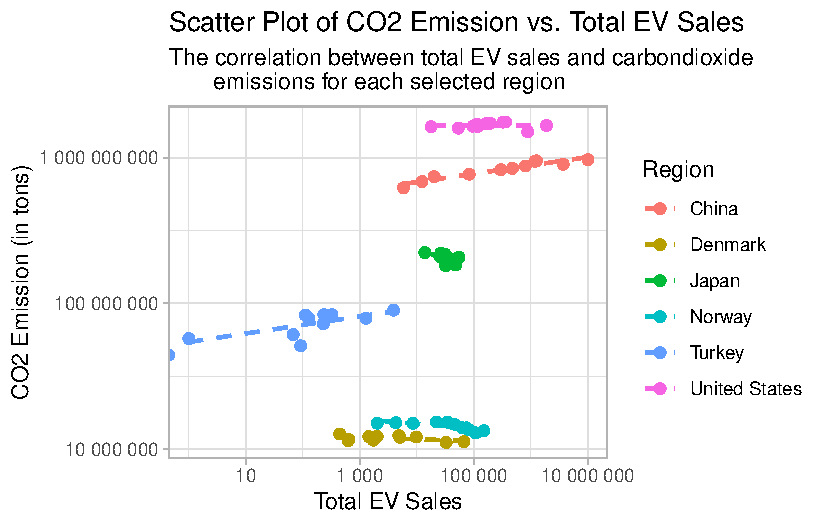
\includegraphics{analysis_files/figure-pdf/unnamed-chunk-16-1.pdf}

The correlation between total sales and carbondioxide emission is
\textbf{not always} positive. \textbf{Half of the countries} has
succeeded to decrease their carbondioxide emissions despite their
increase in the \textbf{total EV sales}.

\section{TURKEY's STATUS (my\_data4)}\label{turkeys-status-my_data4}

\begin{Shaded}
\begin{Highlighting}[]
\FunctionTok{str}\NormalTok{(my\_data4)}
\end{Highlighting}
\end{Shaded}

\begin{verbatim}
tibble [11 x 15] (S3: tbl_df/tbl/data.frame)
 $ year               : chr [1:11] "2011" "2012" "2013" "2014" ...
 $ total              : chr [1:11] "8113111" "8648875" "9283923" "9857915" ...
 $ percentage_total   : chr [1:11] "100" "100" "100.00000000000001" "100.00000000000001" ...
 $ gas                : chr [1:11] "3036129" "2929216" "2888610" "2855078" ...
 $ percentage_gas     : chr [1:11] "37.422500444034348" "33.868173606393896" "31.114109843435799" "28.962290707517766" ...
 $ diesel             : chr [1:11] "1756034" "2101206" "2497209" "2882885" ...
 $ percentage_diesel  : chr [1:11] "21.644397568331065" "24.294558540850687" "26.898208871400591" "29.244368611415293" ...
 $ lpg                : chr [1:11] "3259288" "3569143" "3852336" "4076730" ...
 $ percentage_lpg     : chr [1:11] "40.173097594745101" "41.267135899177639" "41.494700031441454" "41.354890968323424" ...
 $ hybrid             : chr [1:11] "23" "53" "83" "113" ...
 $ percentage_hybrid  : chr [1:11] "0.00028349174564479642" "0.00061279646196759697" "0.00089401861691442287" "0.0011462870191110393" ...
 $ electric           : chr [1:11] "24" "175" "353" "412" ...
 $ percentage_electric: chr [1:11] "0.00029581747371630932" "0.0020233845442326312" "0.0038022719490456778" "0.0041793827599446737" ...
 $ unknown            : chr [1:11] "61613" "49082" "45332" "42697" ...
 $ percentage_unknown : chr [1:11] "0.75942508367012351" "0.56749577257157724" "0.48828496315620024" "0.43312404296446055" ...
\end{verbatim}

\textbf{year:} A character column in my\_data4 data set which represents
the year.

\textbf{total:} A character column in my\_data4 data set which
represents the total number of vehicles that are on traffic.

\textbf{percentage\_total:} A character column which represents the
total number of vehicles over total number of vehicles.

\textbf{gas:} A column in my\_data4 data set which represents the
vehicles which operates with gas.

\textbf{percentage\_gas:} A character column which represents the number
of vehicles that uses gas over total number of vehicles.

\textbf{diesel:} A column in my\_data4 data set which represents the
vehicles which operates with diesel.

\textbf{percentage\_diesel:} A character column which represents the
number of vehicles that are diesel over total number of vehicles.

\textbf{lpg:} A column in my\_data4 data set which represents the
vehicles which operates with LPG.

\textbf{percentage\_lpg:} A character column which represents the number
of vehicles that uses lpg over total number of vehicles.

\textbf{hybrid:} A column in my\_data4 data set which represents the
vehicles which operates with hybrid.

\textbf{percentage\_hybrid:} A character column which represents the
number of vehicles that are hybrid over total number of vehicles.

\textbf{electric:} A column in my\_data4 data set which represents the
vehicles which operates with electric.

\textbf{percentage\_electric:} A character column which represents the
number of vehicles that uses electric over total number of vehicles.

\textbf{unknown:} A column in my\_data4 data set which represents the
vehicles which operates with unknown power.

\textbf{percentage\_unknown:} A character column which represents the
number of vehicles that are unknown over total number of vehicles.

\subsection{Vehicle Trends in Turkey}\label{vehicle-trends-in-turkey}

How about the adoption of \textbf{EV's} and \textbf{the others}
\textbf{in Turkey?}

\textbf{my\_data4} will be used for this part of analysis.

\begin{Shaded}
\begin{Highlighting}[]
\NormalTok{tr\_vehicle\_num }\OtherTok{\textless{}{-}}\NormalTok{ my\_data4 }\SpecialCharTok{|\textgreater{}}
  \FunctionTok{mutate}\NormalTok{(}\FunctionTok{across}\NormalTok{(}\FunctionTok{everything}\NormalTok{(), as.numeric)) }\SpecialCharTok{|\textgreater{}}
  \FunctionTok{select}\NormalTok{(}\SpecialCharTok{{-}}\FunctionTok{starts\_with}\NormalTok{(}\StringTok{"percentage"}\NormalTok{))}

\NormalTok{tr\_vehicle\_num\_long }\OtherTok{\textless{}{-}}\NormalTok{ tr\_vehicle\_num }\SpecialCharTok{|\textgreater{}}
  \FunctionTok{pivot\_longer}\NormalTok{(}
    \AttributeTok{cols =} \FunctionTok{c}\NormalTok{(gas, diesel, lpg, hybrid, electric, unknown), }
    \AttributeTok{names\_to =} \StringTok{"vehicle\_type"}\NormalTok{, }
    \AttributeTok{values\_to =} \StringTok{"value"}        
\NormalTok{  )}

\FunctionTok{head}\NormalTok{(tr\_vehicle\_num\_long)}
\end{Highlighting}
\end{Shaded}

\begin{verbatim}
# A tibble: 6 x 4
   year   total vehicle_type   value
  <dbl>   <dbl> <chr>          <dbl>
1  2011 8113111 gas          3036129
2  2011 8113111 diesel       1756034
3  2011 8113111 lpg          3259288
4  2011 8113111 hybrid            23
5  2011 8113111 electric          24
6  2011 8113111 unknown        61613
\end{verbatim}

Here, the percentage column is deleted, and all other columns of vehicle
types and their values have been brought into columns named
\textbf{vehicle\_type} and \textbf{value} by using
\textbf{pivot\_longer()} function.

In order to visualize the vehicles trend in Turkey, the following code
is used:

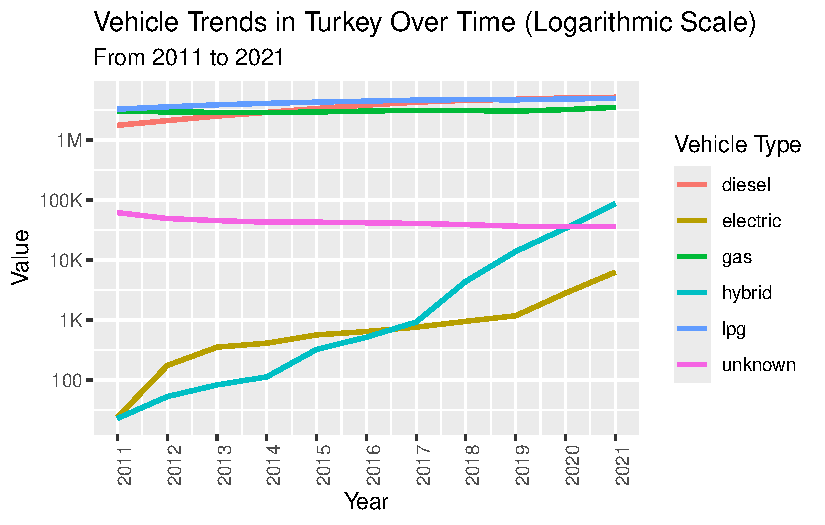
\includegraphics{analysis_files/figure-pdf/unnamed-chunk-19-1.pdf}

Although there was an \textbf{increase} in \textbf{EV's} and
\textbf{hybrid} vehicles, \textbf{Turkey's} total transportation
carbondioxide emission has increased \textbf{consistently} (information
from Country Based Mean Transportation CO2 Emission section) and the
effect of COVID-19 pandemic was quite \textbf{temporary} on it.

The behaviour of the number of vehicles is known now. However, an
important question is, have these increases in the number of \textbf{EV}
and \textbf{hybrid} vehicles been considerable on a proportional view?

\begin{Shaded}
\begin{Highlighting}[]
\NormalTok{vehicle\_prop }\OtherTok{\textless{}{-}} \FunctionTok{c}\NormalTok{(}\StringTok{"percentage\_gas"}\NormalTok{, }\StringTok{"percentage\_diesel"}\NormalTok{, }\StringTok{"percentage\_lpg"}\NormalTok{, }\StringTok{"percentage\_hybrid"}\NormalTok{, }\StringTok{"percentage\_electric"}\NormalTok{, }\StringTok{"percentage\_unknown"}\NormalTok{)}

\NormalTok{tr\_vehicle\_perc\_long }\OtherTok{\textless{}{-}}\NormalTok{ my\_data4 }\SpecialCharTok{|\textgreater{}}
  \FunctionTok{pivot\_longer}\NormalTok{(}\AttributeTok{cols =}\NormalTok{ vehicle\_prop, }\AttributeTok{names\_to =} \StringTok{"vehicle\_type"}\NormalTok{, }\AttributeTok{values\_to =} \StringTok{"percentage"}\NormalTok{) }\SpecialCharTok{|\textgreater{}}
  \FunctionTok{select}\NormalTok{(year, vehicle\_type, }\FunctionTok{starts\_with}\NormalTok{(}\StringTok{"percentage"}\NormalTok{))}

\NormalTok{tr\_vehicle\_perc\_long}\SpecialCharTok{$}\NormalTok{percentage }\OtherTok{\textless{}{-}} \FunctionTok{as.numeric}\NormalTok{(tr\_vehicle\_perc\_long}\SpecialCharTok{$}\NormalTok{percentage)}

\FunctionTok{head}\NormalTok{(tr\_vehicle\_perc\_long)}
\end{Highlighting}
\end{Shaded}

\begin{verbatim}
# A tibble: 6 x 4
  year  vehicle_type        percentage_total percentage
  <chr> <chr>               <chr>                 <dbl>
1 2011  percentage_gas      100               37.4     
2 2011  percentage_diesel   100               21.6     
3 2011  percentage_lpg      100               40.2     
4 2011  percentage_hybrid   100                0.000283
5 2011  percentage_electric 100                0.000296
6 2011  percentage_unknown  100                0.759   
\end{verbatim}

This time, columns including percentages and their values have been
selected brought into columns named \textbf{vehicle\_type} and
\textbf{percentage}, respectively, by using \textbf{pivot\_longer()}
function.

The cumulative bar plot below displays the proportion of vehicle types
over time.

\begin{Shaded}
\begin{Highlighting}[]
\FunctionTok{ggplot}\NormalTok{(tr\_vehicle\_perc\_long, }\FunctionTok{aes}\NormalTok{(}\AttributeTok{x =}\NormalTok{ year, }\AttributeTok{y =}\NormalTok{ percentage,}
                                 \AttributeTok{fill =}\NormalTok{ vehicle\_type)) }\SpecialCharTok{+}
  \FunctionTok{geom\_bar}\NormalTok{(}\AttributeTok{stat =} \StringTok{"identity"}\NormalTok{, }\AttributeTok{position =} \StringTok{"fill"}\NormalTok{, }\AttributeTok{width =} \FloatTok{0.8}\NormalTok{) }\SpecialCharTok{+}
  \FunctionTok{scale\_fill\_brewer}\NormalTok{(}\AttributeTok{palette =} \StringTok{"Paired"}\NormalTok{) }\SpecialCharTok{+}
  \FunctionTok{labs}\NormalTok{(}\AttributeTok{x =} \StringTok{"Year"}\NormalTok{,}
       \AttributeTok{y =} \StringTok{"Percentage"}\NormalTok{,}
       \AttributeTok{title =} \StringTok{"Vehicle Propensity in Turkey Over Time"}\NormalTok{,}
       \AttributeTok{subtitle =} \StringTok{"From 2011 to 2021"}\NormalTok{,}
       \AttributeTok{fill =} \StringTok{"Vehicle Type"}
\NormalTok{  ) }\SpecialCharTok{+}
  \FunctionTok{theme\_tufte}\NormalTok{()}
\end{Highlighting}
\end{Shaded}

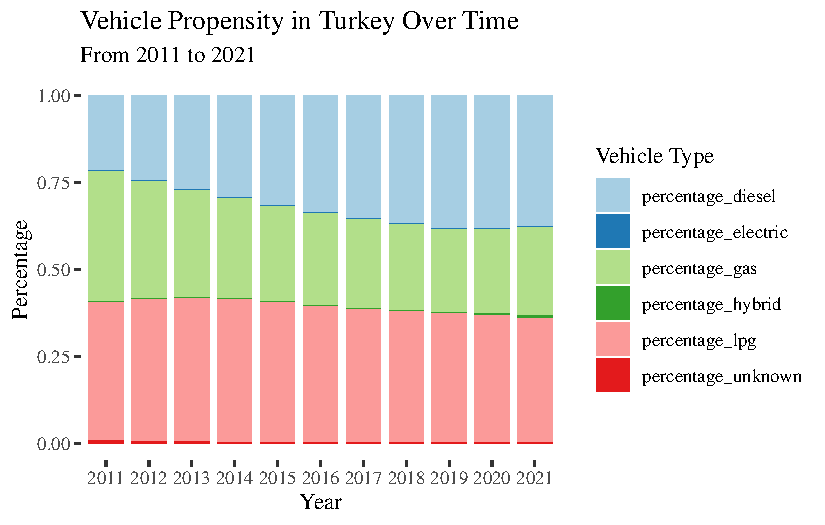
\includegraphics{analysis_files/figure-pdf/unnamed-chunk-21-1.pdf}

In fact, \textbf{non-EV's} were still used widely \textbf{in Turkey},
leading to be the one of the reason of increase in carbondioxide
emission levels.

\section{KEY TAKEAWAYS}\label{key-takeaways}

\begin{itemize}
\item
  \textbf{Electric Vehicles (EV's) and CO2 Emissions:} This study
  examines the impact of EV adoption on CO2 emissions in the
  transportation sector. The analysis covers global EV sales trends and
  CO2 emission levels in various countries over the past decade. • Data
  sources and scope: The analysis uses data from my\_data3, my\_data2,
  and my\_data4, which include information on transportation-related CO2
  emissions, population statistics, and EV sales. The study focuses on
  both global and Turkey-specific trends.
\item
  \textbf{Key Findings:} While countries like China and the United
  States have seen an increase in CO2 emissions, Norway and Denmark have
  demonstrated a decrease in emissions due to strong adoption of
  non-carbon emitting vehicles.
\end{itemize}

Although Turkey has increased the number of electric and hybrid
vehicles, overall CO2 emissions have not significantly decreased,
highlighting the need for infrastructure improvements and greater use of
renewable energy sources.

\begin{itemize}
\item
  \textbf{Factors Influencing Success:} The adoption of electric
  vehicles is most effective when influenced by factors such as
  population density and energy infrastructure.
\item
  \textbf{Main Outcome:} The study concludes that while EV adoption has
  the potential to significantly reduce transportation-related
  emissions, its effectiveness depends on factors such as population
  density and the transition to renewable~energy~sources.
\end{itemize}

\begin{center}
\includegraphics{docs/jaydenj-kirby.gif}
\end{center}




\end{document}
